\documentclass[border=10pt]{standalone}

\usepackage{tikz}
\usepackage{tikzsymbols}
\usetikzlibrary{calc,patterns,shapes.geometric}

\def\centerarc[#1](#2)(#3:#4:#5){\draw[#1] ($(#2)+({#5*cos(#3)},{#5*sin(#3)})$) arc (#3:#4:#5);}

\begin{document}
	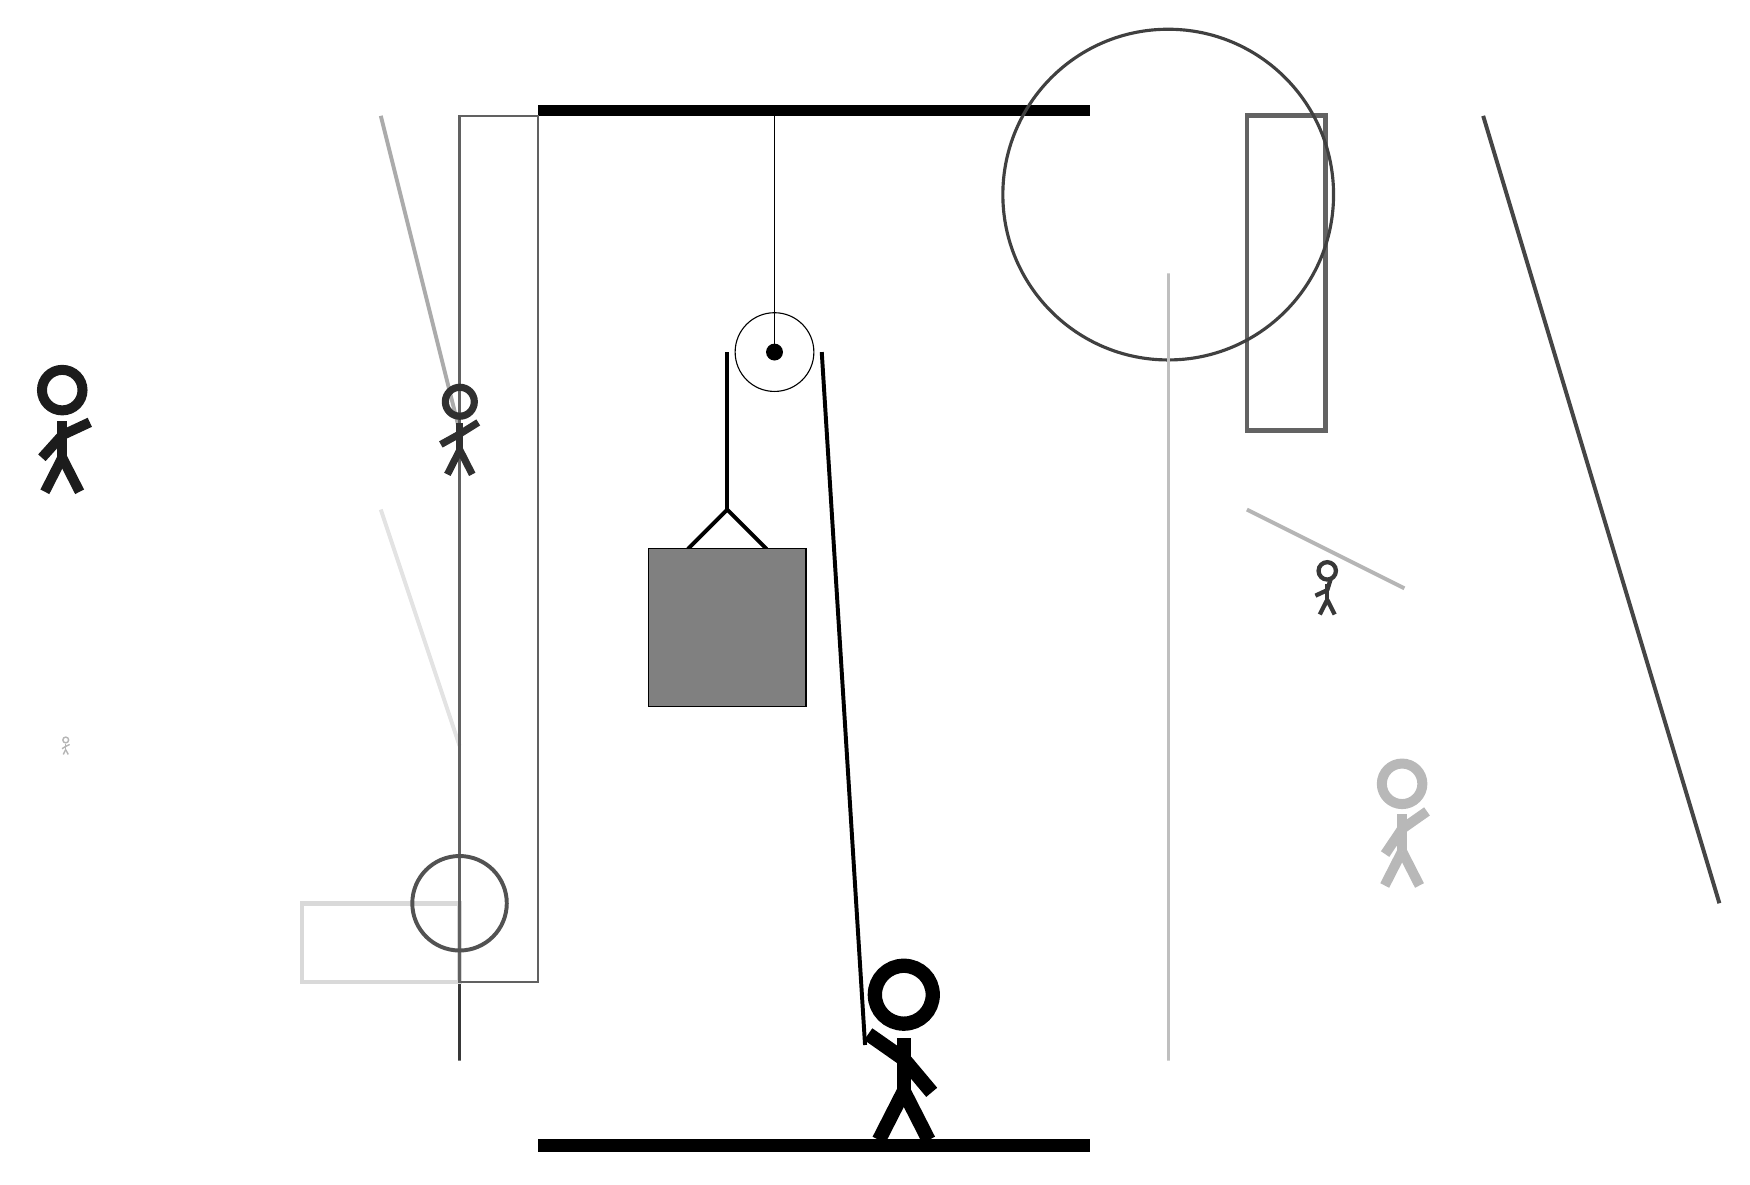
\begin{tikzpicture}
		%%%%% START %%%%%
		
		\draw[fill=black] (-2, 10) rectangle (5, 10.125);
		
		\draw (1, 7) circle (0.5);
		\draw[fill=black] (1, 7) circle (0.1);
		\draw (1, 10) -- (1, 7);
		
		\draw[line width=0.5mm, color=black!73](10, 10) -- (13, 0);
		
		\draw[line width=0.6mm, color=black!61] (7, 10) rectangle (8, 6);
		\draw[line width=0.3mm, color=black!78] (-3, 9) rectangle (-3, -2);
		\draw [line width=0.4mm, color=black!75](6, 9) circle (2.1);
		
		\node[line width=0.5mm, color=black!28] at (9, 1) {\Strichmaxerl[7][56][35]};
		\draw[line width=0.5mm, color=black!11](-3, 2) -- (-4, 5);
		\draw[line width=0.5mm, color=black!33](-4, 10) -- (-3, 6);
		\draw[line width=0.6mm, color=black!15] (-3, 0) rectangle (-5, -1);
		\draw[line width=0.3mm, color=black!62] (-2, 10) rectangle (-3, -1);
		
		\draw [line width=0.5mm, color=black!68](-3, 0) circle (0.6);
		\node[line width=0.3mm, color=black!78] at (8, 4) {\Strichmaxerl[3][25][73]};
		\draw[line width=0.5mm, color=black!29](7, 5) -- (9, 4);
		\node[line width=0.5mm, color=black!81] at (-3, 6) {\Strichmaxerl[5][29][32]};
		
		\node[line width=0.2mm, color=black!29] at (-8, 2) {\Strichmaxerl[1][32][26]};
		\node[line width=0.6mm, color=black!89] at (-8, 6) {\Strichmaxerl[7][48][25]};
		\draw[line width=0.4mm, color=black!25] (6, -2) rectangle (6, 8);
		
		
		\draw[line width=0.5mm] (-0.1, 4.5) -- (0.4, 5.0) -- (0.9, 4.5);
		\draw[fill=black!50] (-0.6, 4.5) rectangle (1.4, 2.5);
		
		\draw[line width=0.5mm] (0.4, 7) -- (0.4, 5.0);
		\centerarc[line width=0.5mm](1, 7)(0:180:0.6);
		\draw[line width=0.5mm](1.6, 7) -- (2.15, -1.8);
		
		\node at (2.6, -1.9) {\Strichmaxerl[10][-35][-50]};
		
		\draw[fill=black] (-2, -3) rectangle (5, -3.15);
		
		%%%%% END %%%%%
	\end{tikzpicture}
\end{document}